\documentclass{report}  
\usepackage[utopia]{mathdesign} 
%\usepackage{amsmath,amsfonts,amsthm,amssymb,mathtools}

\usepackage{forest}

\input{preamble.tex}
\usetikzlibrary{automata, positioning}

\usepackage{amsmath,amsthm,mathtools}
\usepackage{titlesec}
\usepackage{microtype}
\definecolor{myblue}{RGB}{0,82,155}
\usepackage{adjustbox}


%\usepackage[scr]{rsfso}

%\usepackage{libertine}
%\usepackage{mathpazo}
%\usepackage{palatino}
%usepackage{crimson}


\newcommand{\faketarget}{\oplus\!\!\!\!\odot}
\newcommand{\target}{%
  
\begin{tikzpicture}[scale=0.5]
    \fill[black] (0,0) circle (0.1);
    \draw (0,0) circle (0.2);
    \draw (0,0) circle (0.3);
  \end{tikzpicture}%
}

\usepackage[clock]{ifsym}


\title{\Huge{Interface Personne Marchine}\\{IFT2905}\\{\textbf{Introduction}}}
\author{\huge{Franz Girardin}}
\date{\today}
\lstset{inputencoding=utf8/latin1}

            %%%%%%%%%%%%%%%%%  Sect.                          %%%%%%%%%%%%%%%%%%%%%%%%%%%%%%%%%%%%%%%%%%%%%%%%%%%%%%%%%
\usepackage{helvet}
\titleformat{\chapter}[display]
  {\normalfont\bfseries\color{myblue}}
  {\filleft%
    
\begin{tikzpicture}
    \node[
      outer sep=0pt,
      text width=1.5cm,
      minimum height=2cm,
      fill=myblue,
      font=\color{white}\fontsize{40}{50}\selectfont,
      align=center
      ] (num) {\thechapter};
    \node[
      rotate=90,
      anchor=south,
      font=\color{black}\Large\normalfont
      ] at ([xshift=-5pt]num.west) {\textls[180]{\textsc{Section}}};  
    \end{tikzpicture}%
  }
  {5pt}
  {\titlerule[2.0pt]\vskip3pt\titlerule\vskip4pt\large\normalfont}

\titleformat{\section}
  {\normalfont\scshape}{\thesection}{1em}{}



\titleformat{\section}
  {\normalfont\scshape}{\thesection}{1em}{}


% Customizing the spacing for the chapter titles
\titlespacing*{\chapter}{0pt}{0pt}{20pt}

%\usepackage[utopia]{mathdesign}
% Allow hfill in math environment
\newcommand{\specialcell}[1]{\ifmeasuring@#1\else\omit$\displaystyle#1$\ignorespaces\fi}

% Allow you to do the non implication (implication barred)
\newcommand{\notimplies}{%
  \mathrel{{\ooalign{\hidewidth$\not\phantom{=}$\hidewidth\cr$\implies$}}}}



\DeclareRobustCommand{\looongrightarrow}{%
  \DOTSB\relbar\joinrel\relbar\joinrel\relbar\joinrel\rightarrow
}


\title{\Huge{Interface PM}\\{IFT2905}\\{\textbf{Feuille de notes}}}
\author{\huge{Franz Girardin}}
\date{\today}


\begin{document}
\maketitle
\pagebreak
\tableofcontents
\pagebreak
\begin{multicols*}{3}


    \footnotesize
    \paragraph{Style de language de programmation} 

    \chapter{Extended Backus-Naur Form}

\begin{Definitionx}{EBNF}{}
  Une \textbf{grammaire} qui fournit un façon d'exprimer formellement 
  la \textbf{structure} d'un langage. 
  \mbox{}
  \\ \\ 
  $\blacktriangleright$  \textbf{ Clarifie} et communique la struct. 
\end{Definitionx}


\begin{align*}
  \texttt{Lang. prog. } & \Coloneqq \bigl\{\text{symboles} \bigr\}   
  \hookrightarrow \bigl\{ \text{phrase} \bigr\} 
  \\
  \texttt{Vocabulaire} & \Coloneqq \sum \text{phrases}
  \\
  \texttt{Grammaire} & \Coloneqq \bigl\{ \text{Règles} \; \big| \;
              \texttt{règle} = f(\texttt{symbole})  \bigr\}
\end{align*}      

\begin{Definitionx}{Grammaire}{}
    La \textbf{grammaire} est l'ensemble des \texttt{règles} 
    de \textbf{syntaxe} qui spécifie l'usage adéquat du langage   
\end{Definitionx}

En \textbf{BNF},   un langage de programmation $L(G)$ est un 
\textbf{ensemble} composé d'éléments $p$ tels 
qu'il est possible d'utiliser un élément de départ 
\texttt{dp} et une série de \textbf{règle de production} 
pour obtenir un nouvel élément $p$. 

\begin{align*}
    L(G) = \bigl\{ \langle p \rangle \; | \; \texttt{dp}    
              \hookrightarrow \cdots \hookrightarrow p
    \rangle  \bigr\}
\end{align*}

\begin{EExample}{Définition d'une catégorie en \textbf{BNF}  }{}
    \begin{align*}
      &\texttt{\textit{\textcolor{myb}{// Une catégirie composée d'élem. }}}
      \textcolor{myb}{x_i}  
      \\
      &\langle \texttt{cat}  \rangle \Coloneqq x_1 x_2 \cdots x_n  
      \\
      \\
      & \langle \texttt{bin} \rangle \Coloneqq 0 
      \\
      & \langle \texttt{bin} \rangle \Coloneqq 1 
      \\
      &\texttt{\textit{\textcolor{myb}{// Règle production 
      d'un nouveau binaire}}}
      \\
      &\langle \texttt{bin} \rangle \Coloneqq \langle \texttt{bin} \rangle 
                       \langle \texttt{bin} \rangle 
      \\ 
      \\ 
      &\texttt{\textit{\textcolor{myb}{// Application d'une règle de production}}}
      \\
      &\langle \texttt{bin} \rangle \Coloneqq \langle \texttt{bin} \rangle 
                       \langle \texttt{bin} \rangle 
      \hookrightarrow \langle \texttt{bin} \rangle 0  
      \hookrightarrow 1 \; 0 
    \end{align*}
\end{EExample}

\begin{Definitionx}{Grammaire ambigue}{}
   $G$ est ambigue s'il $p \in L(G)$ tel que $p$ a plus d'un 
   \textit{parse tree} ou 
   \textbf{arbre de dérivation}. 
\end{Definitionx}


\begin{EExample}{Expression ambigue $x - x - x$}{}
 \textbf{Arbre de dérivation 1} :  
 \mbox{}\\\\
 \begin{forest}
  for tree={math content, s sep=7mm, inner sep=0.1em}
  [<\texttt{expr}>
    [<\texttt{expr}>
      [x]
    ]
    [-]
    [<\texttt{expr}>
      [<\texttt{expr}>
        [x]
      ]
      [-]
      [<\texttt{expr}>
        [x]
      ]
    ]
  ]
\end{forest}

 \textbf{Arbre de dérivation 2} :  
 \mbox{}\\\\
\hspace{1cm}
\begin{forest}
  for tree={math content, s sep=4mm, inner sep=0.1em}
  [<\texttt{expr}>
    [<\texttt{expr}>
      [<\texttt{expr}>
        [x]
      ]
      [-]
      [<\texttt{expr}>
        [x]
      ]
    ]
    [-]
    [<\texttt{expr}>
      [x]
    ]
  ]
\end{forest}   
\end{EExample}


\begin{Definitionx}{Arbre de syntaxe abstraite (ASA)}{}
  Structure \textit{ hiérarchique} qui représente la 
  \textbf{structure syntaxique} abstraite d'une expression.   
\end{Definitionx}

\begin{EExample}{ASA d'expr. conditionnelle}{} 
  Soit l'expression suivante 
\begin{lstlisting}
   if (x < y) then :
    x := y + 1
\end{lstlisting}

On a l'\textbf{ASA}  :
\begin{center}
    \begin{forest}
for tree={font=\ttfamily, reversed}
  [if-then
    [assign
      [x]
      [+ 
        [y]
        [1]
      ]
    ]
    [<
      [x]
      [y]
    ]
  ]
\end{forest}   
\end{center}
\end{EExample}

% Song : look how far we've made it. We're still together, still 
% going strong


\begin{Definitionx}{Diagramme syntaxique}{}
  Il s'agit d'une représentation \textbf{graphique} 
  d'une \textit{règle de syntaxe} 
  qui permet de visualiser l'\textbf{arrangement des symboles} terminaux 
  et non terminaux. 

\end{Definitionx}

\begin{EExample}{Diagramme syntaxique d'un flottant}{}
  \begin{adjustbox}{width=\linewidth}
    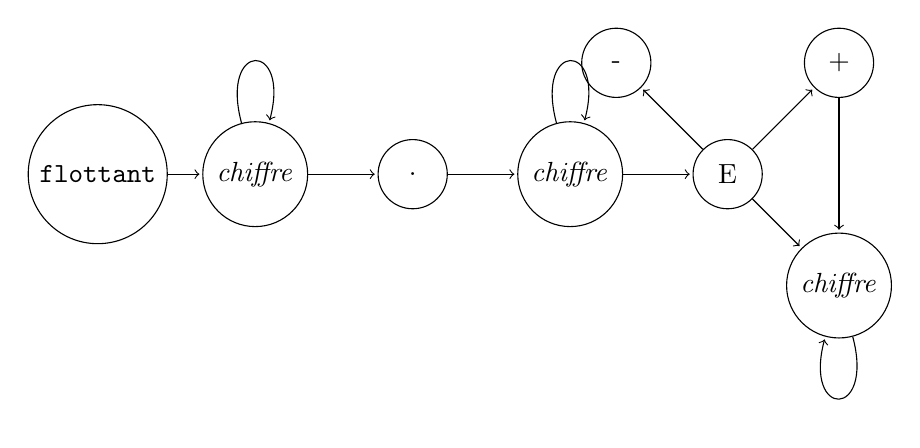
\begin{tikzpicture}[shorten >=1pt, node distance=2cm, on grid, auto]

      % Nodes for the floating point number
      \node[state] (init) {\texttt{flottant}};
      \node[state] (chiffre1) [right=of init] {\textit{chiffre}};
      \node[state] (dot) [right=of chiffre1] {.};
      \node[state] (chiffre2) [right=of dot] {\textit{chiffre}};
      \node[state] (e) [right=of chiffre2] {E};
      \node[state] (sign) [above right=of e] {+};
      \node[state] (signneg) [above left=of e] {-};
      \node[state] (chiffre3) [below right =of e] {\textit{chiffre}};
      

      % Edges for the floating point number
      \path[->]
        (init) edge node {} (chiffre1)
        (chiffre1) edge [loop above] node {} (chiffre1)
        (chiffre1) edge node {} (dot)
        (dot) edge node {} (chiffre2)
        (chiffre2) edge [loop above] node {} (chiffre2)
        (chiffre2) edge node {} (e)
        (e) edge node {} (sign)
        (e) edge node {} (signneg)
        (e) edge node {} (chiffre3)
        (sign) edge node {} (chiffre3)
        (chiffre3) edge [loop below] node {} (chiffre3);

     \end{tikzpicture}
  \end{adjustbox}
\end{EExample}







  \end{multicols*}
\end{document}
